\chapter{Probability}

\section{Basic concepts and results}

A \textbf{random experiment} is when a set of all possible outcomes is known, but it is impossible to predict the actual outcome of the experiment.
A \textbf{sample space}, denoted as $\Omega$, contains all possible outcomes of the experiment.
An \textbf{event} is a subset of $\Omega$. We say that $A\subset\Omega$ has occrred if and only if the outcome of the experiment is an element of $A$. 
Formally, the family of events forms a $\sigma$-algebra of subsets of $\Omega$ that we denote by $\mcA$.
\nt{
    \begin{itemize}
        \item $\Omega\in\mcA$
        \item $A\in\mcA\Rightarrow\bar{A}\in\bar{\mcA}$ ,where $\bar{A}$ indicates the compliment of A
        \item $A_1, A_2,\cdots\in\mcA$
        \item $\displaystyle\bigcup_{i=1}^{\infty}A_i\in\mcA$
    \end{itemize}
}
\subsection{Probability measures}
\dfn[]{Kolmogorov's axioms}{
    \begin{itemize}
        \item $P(A)\geq 0$
        \item $P(\Omega)=1$
        \item If $A_i\bigcap A_j = \emptyset, i\neq j$, then $P(\cup_i A_i) = \sum_i P(A_i)$
    \end{itemize}
}

Probability measure $P: \mcA\to\bbR$ satisfying Kolmogorov's axioms has the following properties:
\begin{itemize}
    \item $P(\varnothing) = 0$
    \item $A\subset B\Rightarrow P(A) \leq P(B)$
    \item $0\leq P(A)\leq 1$
    \item $P(A\cup B) = P(A) + P(B) - P(A\cap B)$
    \item $P(\bar{A}) = 1 - P(A)$
    \item $P(A-B) = P(A\cap \bar{B}) = P(A) - P(A\cap B)$
\end{itemize}

\dfn[]{Conditional probability}{
    If $P(B) > 0$,\\

    $\displaystyle P(A|B)=\frac{P(A\cap B)}{P(B)}$\\

    We are re-evaluating the probability of A given the B space.
}\bigskip

Let $\{A_1, A_2,\cdots\}$ denote a partition of $\Omega: \cup_i A_i = \Omega$; $A_i\cap A_j = \emptyset, i\neq j$.
Meaning union makes up $\Omega$ and are mutually exclusive. Then if $P(A_i)>0$ for all $i$
\thm[]{Total probability theorem}{
    $P(B) = \displaystyle \sum_i P(B|A_i)P(A_i)$
}
$B = B\cap \Omega = B\cap [\cup_i A_i] = \cup_i (B\cap A_i)$ and $P(\cup_i B\cap A_i) = \sum_i P(B\cap A_i)$
\thm[]{Bayes' theorem}{
    If $P(B)>0$\\

    $\displaystyle P(A_i|B) = \frac{P(B|A_j)P(A_j)}{\sum_i P(B|A_i)P(A_i)}$
}
$\displaystyle P(\underbrace{A_j}_{\text{explanation}}|\underbrace{B}_{\text{evidence}}) = \frac{P(A_j \cap B)}{P(B)} = \frac{P(B|A_j)P(A_j)}{\underbrace{P(B)}_{\text{substitute with total probability theorem}}}$

\subsection{Random variables}
\dfn[]{Random variable}{
    Function defined in $\Omega$ and taking values in $\bbR$\\

    $X: \Omega\to\bbR$\\

    $\omega\mapsto X(\omega) = x$
}
A random variable induces a probability measure in $\bbR$ that we denote by $P_X$: if $B\subset\bbR$,
$P_X(B) = P(A)$, where $A = X^{-1}(B) = \{\omega\in\Omega: X(\omega)\in B\}$.
Formally, there must be a $\sigma$-algebra of subsets of $\bbR$,$\mcB$, and we have to verify that for every set $B\in\mcB$ we have $X^{-1}(B)\in\mcA$.
Typically, $\mcB$ is the so called Borel $\sigma$-algebra and it suffices to make sure that X satisfies $X^{-1}((-\infty,x])\in\mcA$ ,$\forall x\in\bbR$.
\\

Basically what it means is that we don't know if $X^{-1}(B)\in\mcA$ and for which B can I compute $P_X(B)$.
If $X^{-1}(B)\in\mcA$ for B is in the Borel $\sigma$-algebra, then X is measurable.

\dfn[]{Distribution function of a random variable}{
    X: for all $x\in\bbR$\\

    $F_X(x) = P_X((-\infty,x]) = P(X\leq x)$
}
It is suffice to know $F_X(\cdot)$ to be able to compute $P_X(B)$ for all $B\in\mcB$.
\begin{itemize}
    \item For all $a>b$, $P(a<X\leq b) = F_X(b) - F_X(a)$
    \item $F_X(-\infty)=0$; $F_X(\infty)=1$
    \item $F_X$ is right-continuous and non-decreasing
    \item The set of points at which $F_X$ is discontinuous is either finite or countable (at most countable)
\end{itemize}

\dfn[]{Discrete random variable}{
    X is a discrete random variable if $D_X$ is such that $P_X(D_X)=1$
}
The probability mass function of X is defined as 
$\displaystyle f_X(x) = F_X(x) - \lim_{y\to x}F_X(y) = \begin{cases}
    P(X=x) & \text{if }x\in D_X\\
    0 & \text{otherwise}
\end{cases}$\\
Any $f$ satisfying the following is a probability mass function
\begin{itemize}
    \item $f(x)\geq 0$ for all $x$
    \item $f(x)>0$ iff $x\in D$, where $D\subset\bbR$ is finite or countable
    \item $\sum_{x\in D} f(x) = 1$
\end{itemize}
For any event $B\subset\bbR, P(X\in B) = \displaystyle \sum_{x\in B\cap D_X}f_X(x)$.
\nt{
    $F_X(x) = \sum_{y\leq x}f_X(y)$\\

    $F_X(x) = P(X\leq x)$ cumulative distribution function\\
    $\downarrow$\\
    $f_X(x) = P(X=x)$ probability mass function\\
    where $0\leq f_X(x) \leq 1$
}
Discrete distribution include Bernoulli, binomial, Poisson, geometric, negative binomial, multinomial, hypergeometric, etc.

\dfn[]{Continuous random variable}{
    X is continuous if $P_X(D_X)=0, D_X = \varnothing$ and if additionally there is $f_X$ such that for all $x\in\bbR$
    \begin{itemize}
        \item $f_X(x)\geq 0\rightarrow$ probability density function
        \item $F_X(x) = \int_{-\infty}^{+\infty}f(x)\,dx = 1$
    \end{itemize}
}
At the points where $F_X$ is differentiable, we have $F'_X(x) = f_X(x)$.\\

Any $f$ satisfying the following conditions is a probability density function
\begin{itemize}
    \item $f(x)\geq 0$ for all $x$
    \item $\int_{-\infty}^{+\infty}f(x)\, dx =1$
\end{itemize}
Continuous distributions include uniform, exponential, gamma, chi-squared, normal. $t$-student, $F$-Snedcor, beta, Pareto, Weibull, log-normal, etc.

\subsection{Functions of a random variable}
Let $X$ be a r.v. and $Y=h(X)$ where $h:\bbR\to\bbR$\\
In general, if $X=g(Y)$ with $g$ invertible and differentiable, and $X$ continuous, we have
    \begin{center}
        $f_Y(y) = |g'(y)|\, f_x(g(y))$
    \end{center}
\begin{proof}
    $\displaystyle\frac{\partial F_X(x)}{\partial x}=f_X(x)$\\
    Using chain rule: $(f\circ g)'(x) = [f(g(x))]' = f'(g(x))g'(x)$
\end{proof}
\dfn[]{Expected value}{
    Let $Y = h(X)$, a linear function.\\
    
    The expected value of Y is defined by
    $\displaystyle E[Y]=
    \begin{cases}
        \sum_x h(x)\, f_X(x) & \text{if $X$ discrete}\\
        \int_{-\infty}^{+\infty}h(x)\, f_X(x)\, dx & \text{if $X$ continuous}
    \end{cases}$\\

    Formally, we must addtionally verify that the integral or series are absolutely convergent.
    $E[Y]$ may not exist.
}

There are two ways to compute $E[Y]$ with $Y=h(X)$, either use the definition above, or first obtain the distribution of $Y$
and compute
$\displaystyle E[Y] = 
\begin{cases}
    \sum_{y}y\, f_Y(y) & \text{if $Y$ discrete}\\
    \int_{-\infty}^{+\infty}y\ f_Y(y)\, dy & \text{if $Y$ continuous}
\end{cases}$. The two methods are equivalent.
\dfn[]{Raw moment of oder $k$}{
    $\mu'_k = E[X^k]$
}
\dfn[]{Central moment of order $k$}{
    $\mu_k=E[(X-\mu)^k]$, $\mu=E[X]$
}
\dfn[]{Moment generating function}{
    $M_X(s) = E[e^{sX}]$ whenever the expectation exists for $s$ in a neighborhood of the origin.
}
\begin{itemize}
    \item If $M_X(s)$ exists, then $X$ has moments of all orders and $M^{(k)}(0) = E[X^k]$
    \item The moment generating function, when it exists, identifies the probability distribution
\end{itemize}
Some useful \textbf{properties}:
\begin{itemize}
    \item $E[h_1(X) + h_2(X)] = E[h_1(X)] + E[h_2(X)]$
    \item If $c\in\bbR$, then $E[cX] = cE[X]$; $E[c] = c$
    \item If $c\in\bbR$, then $Var(cX+b)=c^2Var(X)$
    \item $Var(X) = E[X^2]-(E[X])^2$
    \item $Var(X)\geq 0$; $Var(X) = 0\Leftrightarrow P(X=c)=1$ for some $c\in\bbR$
\end{itemize}

\subsection{Bivariate random variables}

\begin{equation*}
\begin{split}
    (X,Y): & \,\Omega\to\bbR^2\\
        & \,\omega\mapsto(X(\omega),Y(\omega))=(x,y)
\end{split}    
\end{equation*}

If $(X,Y)$ discrete, we define the joint probability mass function as $f(x,y) = P(X=x, Y=y)$. 
If $(X;Y)$ continuous, then there exists the joint probability density function, $f(x,y)$
such that for all $(x,y)\in\bbR^2$,
\begin{itemize}
    \item $f(x,y)\geq 0$
    \item $F(x,y)=P(X\leq x, Y\leq y) = \int_{-\infty}^{x}\int_{-\infty}^{y}f(u,v)\, dv\, du$
\end{itemize}
\ex[]{}{
    X = weight, Y = height $\Rightarrow$ Z = BMI
}
\dfn[]{Marginal distributions}{
    $f_X(x) =
    \begin{cases}
        \sum_y f(x,y) & \text{if $(X,Y)$ discrete}\\
        \int_{-\infty}^{+\infty}f(x,y)\, dy & \text{if $(X,Y)$ continuous}
    \end{cases}$
}
\dfn[]{Expectation of $Z=h(X,Y)$}{
    $E[Z] = \begin{cases}
        \sum_x\sum_y h(x,y)\, f(x,y) & \text{if $(X,Y)$ discrete}\\
        \int_{-\infty}^{+\infty}h(x,y)\, f(x,y)\, dy\, dx & \text{if $(X,Y)$ continuous}
    \end{cases}$
}
\dfn[]{Conditional didstributions}{
    $f_{X|Y=y}(x)=\frac{f(x,y)}{f_Y(y)}$, $y$ fixed: $f_Y(y)>0$\\

    function of $x$ for every $y$ where $f_Y(y)>0$
}
\dfn[]{Raw moment of order $(r,s)$}{
    $\mu'_{(r,s)}=E[X^r\,Y^s]$
}
\dfn[]{Central moment of order $(r,s)$}{
    $\mu_{(r,s)}=E[(X-\mu_X)^r\,(Y-\mu_Y)^s]$
}
\dfn[]{Covariance}{
    Cov$(X,Y) = E[(X-\mu_X)(Y-\mu_Y)] = \mu_{(1,1)}$
}
If $x$ and $y$ are positively associated $\rightarrow$ Cov$(x,y)>0$ $\rightarrow$ If $x$ is larger than its mean, then typically $y$ is larger than its mean.\\

Some useful \textbf{properties}:
\begin{itemize}
    \item Cov$(X,Y) = E[X,Y] - E[X]E[Y]$
    \item Cov$(X,Y) = \text{Cov}(Y,X)$
    \item Cov$(cX,Y) = c\text{Cov}(X,Y), c\in\bbR$
    \item Cov$(X+Y, Z) = \text{Cov}(X,Z)+\text{Cov}(Y,Z)$
    \item Var$(X\pm Y) = \text{Var}(X)+\text{Var}(Y)\pm 2\,\text{Cov}(X,Y)$
\end{itemize}
\ex[]{Portfolio management}{
    Cov$(x,y) <0$\\
    Var$(x,y) < \text{Var}(x)+\text{Var}(y)$
}

\thm[]{Law of iterated expectation}{
    If $Z = h(X,Y)$ then $E[Z] = E_X[E[Z|X]]$
}
\thm[]{Law of total variance}{
    Var$(Y) = \text{Var}_X(E[Y|X])+E_X[\text{Var}(Y|X)]$
}
Other useful tricks:
\begin{itemize}
    \item $E[h(X)\,Y\,|\,X=x] = h(x)\, E[Y\, | \, X=x]$
    \item Cov$(X,Y) = \text{Cov}(X,E[Y|X])$
    \begin{proof}
        \begin{equation*}
        \begin{split}
            \text{Cov}(X,E[Y|X]) & = E[X\,E[Y|X]]-E[X]\,E[E[Y|X]]\\
            & = E[E[XY|X]]-E[X]\,E[Y]\\
            & = E[XY]-E[X]\,E[Y]\\
            & = \text{Cov}(X,Y)
        \end{split}
        \end{equation*}
    \end{proof}
\end{itemize}

\subsection{Independence}
\dfn[]{Stochastic independence}{
    $X$ and $Y$ are stochastically independent if and only if $\forall(x,y)\in\bbR^2$, $f(x,y)=f_X(x)\, f_Y(y)$
}
If $X$ and $Y$ are independent, then
\begin{itemize}
    \item Var$(X+Y) = \text{Var}(X) + \text{Var}(Y)$
        \begin{proof}
            Var$(X\pm Y)=\text{Var}(X)+\text{Var}(Y) \pm 2\times \underbrace{\text{Cov}(X,Y)}_{\rightarrow 0}$
        \end{proof}
    \item $M_{X+Y}(s) = M_X(s)\,M_Y(s)$
        \begin{proof}
            $M_{X+Y}(s) = E[e^{s(X+Y)}] = E[\underbrace{e^{sx}}_{u}\underbrace{e^{sy}}_{v}]$\\

            $x$ and $y$ independent stochastically $\Rightarrow$ $u$ and $v$ independent\\

            $M_{X+Y}(s) = E[e^{sx}]\,E[e^{sy}] = M_X(s)\,M_Y(s)$
        \end{proof}
    \item Cov$(X,Y) = 0$
        \begin{proof}
            Cov$(X,Y) = E[(X-\mu_X)(Y-\mu_Y)] = \underbrace{E[XY]}_{X, Y \text{uncorrelated}}-\,E[X]E[Y]=E[X]E[Y]-E[x]E[Y]=0$
        \end{proof}
    \item $E[X^r Y^s] = E[X^r]\, E[Y^s]$
    \item $E[Y\,|\,X=x] = E[Y]$; $E[X\, |\, Y=y] = E[X]$
    \item $f_{X|Y=y}(x)=f_X(x)$; $f_{Y|X=x}(y)=f_Y(y)$
        \begin{proof}
            $\displaystyle f_{X|Y=y}(x) = \frac{f(x,y)}{f_Y(y)} = \frac{f_X(x)f_Y(y)}{f_Y(y)}=f_X(x)$
        \end{proof}
\end{itemize}
\dfn[]{Mean independence}{
    $Y$ is mean independent of $X$ iff $E[Y\,|\,X=x]$ does not depend on $x$ for all $x$.
}
\begin{proof}
    $E[Y|X=x] = c$\\

    $E[Y|X] = c \Rightarrow E[E[Y|X]] = c \Rightarrow E[Y]=c\rightarrow$ conditional is equal to marginal
\end{proof}

\dfn[]{Uncorrelatedness}{
    $X$ and $Y$ are uncorrelated iff Cov$(X,Y) = 0$
}
Useful \textbf{results}:
\begin{itemize}
    \item If $X$ and $Y$ are stochastically independent, then $Y$ is mean-independent of $X$, and $X$ is mean independent of $Y$.
    \item If $Y$ is mean-independet of $X$, then $X$ and $Y$ are uncorrelated. The converse is not true.
        \begin{proof}
            $Y$ mean independence of $X \Rightarrow \text{Cov}(X,Y) = \text{Cov}(X, E[Y|X]) = \text{Cov}(X,c) = 0\Rightarrow$ uncorrelated
        \end{proof}
    \item If $Y$ is uncorrelated with $X$, then $E[XY] = E[X]E[Y]$
    \item If $Y$ is mean-independent of $X$, then $E[X^k Y]=E[X^k]E[Y]$ for all $k$
    \item If $Y$ and $X$ are stochastically independent, then $E[X^k Y^r] = E[X^k]E[Y^r]$ for all $k,r$
\end{itemize}
\nt{
    stochastic independence $\Rightarrow$ mean independence $\Rightarrow$ uncorrelatedness
}

\section{Convergence of sequences of random variables}

\begin{itemize}
    \item Notions of Convergence
        \begin{enumerate}
            \item Pointwise convergence
            \item Uniform convergence
            \item Convergence in $L^P$
            \item Convergence in measure
        \end{enumerate}
    \item Convergence for random variables
        \begin{enumerate}
            \item Almost surely
            \item In the $r$th mean
            \item In probability
            \item In distribution
        \end{enumerate}
    \item Skorokhod representation theorem
    \item Continuous mapping theorem
    \item Slutsky theorem
\end{itemize}

\subsection{Notions of convergence}
If $\{X_n\}_{n=1}^{\infty}$ is a sequence of random variables and $X$ is a random variable,
\begin{equation*}
    \begin{split}
        X_n : &\underbrace{\Omega}_{\text{exists probability, $\sigma$-algebra}}\to\bbR\\
        &X_n\longrightarrow X \qquad \text{as } n\rightarrow +\infty
    \end{split}     
\end{equation*}
$n$ can be population size, or can be the number of iterations for Monte Carlo simulation.\\

Notions of \textbf{convergence}: let $f_n, f : [0,1]\to\bbR$
    \begin{itemize}
        \item Point wise convergence: $f_n(x)\to f(x)$ for all $x\in[0,1]$
        \item Uniform convergence: $\displaystyle\sup_{x\in[0,1]}|f_n(x)-f(x)|\to 0$
        \item Convergence in $L^P$: $\displaystyle\int_{0}^{1}|f_n(x)-f(x)|^P\, dx\to 0$
        \item Convergence in measure: $\mu(A_{n,\epsilon})\to 0$ for all $\epsilon>0$ where $A_{n,\epsilon}=\{x\in[0,1] : |f_n(x)-f(x)|>\epsilon\}$
    \end{itemize}

\ex[]{}{
    $f_n : [0,1]\to\bbR$\\

    $\displaystyle f_n(x)=
    \begin{cases}
        0 & 1/n \leq x \leq 1\\
        n-n^2 x & 0\leq x < 1/n
    \end{cases}$\bigskip\\

    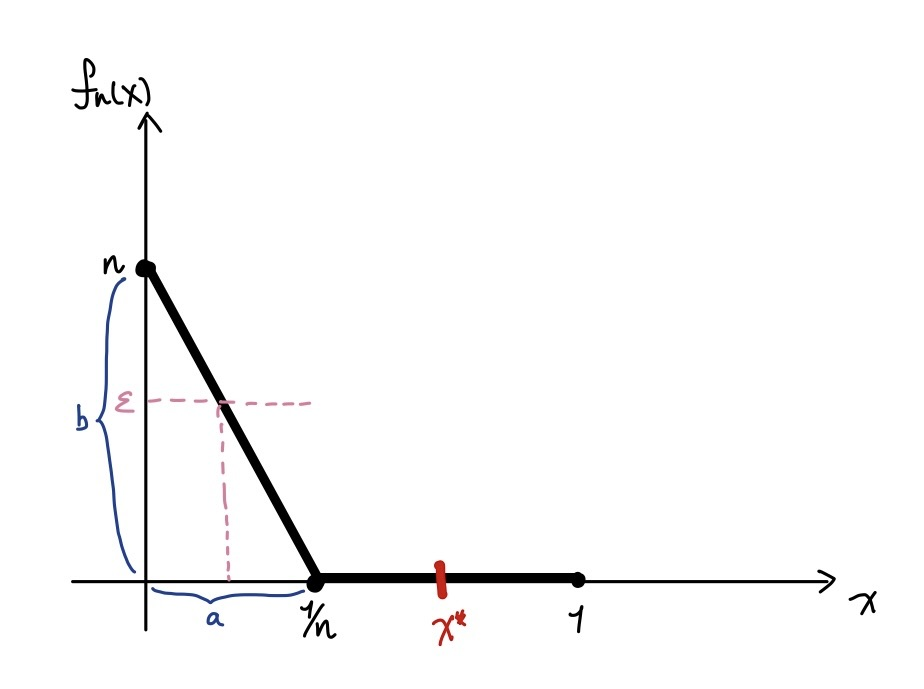
\includegraphics[scale=0.2]{Images/1.jpg} As $n\to\infty$, a becomes smaller, b becomes bigger.\\

    \begin{itemize}
        \item Point wise convergence
            \begin{equation*}
                \forall x\in [0,1]\\
                
                \forall x^* > 0, f_n(x^*)=0\qquad\text{for } n>N\qquad\text{except } f_n(0)=0 \to\infty\\

            \end{equation*}
        \item Uniform convergence
        \item Convergence in $L^1$
        \item Convergence in measure
    \end{itemize}
}

\section{Important asymptotic results}

\begin{itemize}
    \item Weak law of large numbers
    \item Strong law of large numbers
    \item Central limit theorem
    \item Lévy's continuity theorem
    \item Applications
        \begin{enumerate}
            \item Bernoulli
            \item Simple Monte Carlo
        \end{enumerate}
    \item Delta method and its applications
        \begin{enumerate}
            \item Log odds
            \item Variance stabalizing
        \end{enumerate}
\end{itemize}